\documentclass[14pt]{extreport}
\usepackage{gost}
\usepackage{lscape}
\usepackage{lscape}
\usepackage[justification=centering]{caption}
\usepackage{diagbox}
\usepackage{graphics}
\usepackage{alltt}
%Тут можно вставить дополнительные пакеты

\setstretch{1.5}
\begin{document}
\pagestyle{empty} %  выключаем нумерацию

\includepdf[pages=-,pagecommand={}]{titleCourse.pdf}

\setcounter{page}{1}
 %  выключаем нумерацию
\tableofcontents

\intro
\pagestyle{plain} % включаем нумерацию
\setcounter{page}{1}
В современном мире людям всё важнее и важнее удобство и скорость. Любой человек, когда заказывает предметы из интернет магазина, не будет ждать долгой загрузки сайта. Такие ситуации раздражают покупателя и увеличивает вероятность того, что он обратится к другому интернет магазину.
Кроме того, сейчас всё больше людей после самоизоляции из-за COVID-19 продолжают пользоваться доставкой. Это удобно, так как много людей разобрались с работой доставки и теперь по желанию и возможности пользуются такой функцией. 

Всё это мотивирует создавать всё больше быстрых, отзывчивых интернет-магазинов с функцией доставки. Рассмотрим статистику за 2022 год роста онлайн-продаж. Исходя из статистики можно сделать вывод, что рост онлайн продаж только растёт, и в категориях не хватает увеличения онлайн продаж продуктов других категорий таких, как например овощи и фрукты. С такой категорией связана проблема, малый срок годности и большинство людей предпочитают самому рассматривать такие товары и определять по их внешнему виду качество, однако на данный момент всё больше людей пытаются заказывать подобные товары.

Исходя из данного анализа, можно сделать вывод, что интернет-магазин фруктов будет востребованным, если у него будет хорошо сделана логическая модель базы данных, это позволит быстрее загружать товары и заказы. Кроме того, в таком магазине необходимо создать связь между сотрудниками и клиентами, так как именно доверие сотруднику позволит купить фрукты, не рассматривая их внешний вид самому. Сотрудник дружелюбно и вежливо будет общаться с клиентом: отвечать на вопросы и рассказывать о качестве товаров, выстраивая доверительные отношения.

Таким образом интернет-магазин фруктов станет актуальнее и доступнее, и всё больше людей не имеющих возможности или желания самому прийти за товарами, смогут заказывать скоропортящиеся, редкие и качественные фрукты.

Целью данной работы является создание базы данныый, и реализация запросов к ней.

Для достижения данно цели были поставлены следующие задачи:
\begin{enumerate}
    \item Определить новый функционал.
    \item Создать логическую модель базы данных.
    \item Преобразовать логическую модель в физическую.
    \item Создать SQL запросы для получения данных. 
\end{enumerate}


\chapter{Создание углубленного сценария использования базы данных.}

В данном разделе будет представлен углубленный сценарий использования базы данных магазина по продаже овощей и фруктов.


Магазин овощей и фруктов предоставляет возможность продажи как в розницу так и в формате интернет-магазина. У магазина два варианта покупателей: Анонимный пользователь и зарегистрированный в системе. Анонимным пользователем является человек, который произвел покупку без авторизации в системе. Например: если покупка была произведена в физическом магазине без использования программы лояльности, или же без авторизации в онлайн-магазине. Внутри системы существует роль продавца-консультанта, который может вносить данные о заказах, которые оформляет пользователь. Если заказ был произведен онлайн, то данные о заказе вносится автоматизированной системой. Дальнейшее сопровождение заказа выполняется при помощи продавцов-консультантов. В штате компании существует складской работник, который взаимодействует с товарами на складе. Он оперирует с занесением полученным от поставщиков продуктов, также следит за сроками годности позиций на складе (существует отдельное предоставление). Для автоматизированной системы существует представление (view) которое возвращает вычисленные данные (оставшийся срок годности от партии, базовая стоимость, стоимость со скидкой) для отображения на клиенте онлайн-магазина.

\chapter{Определение ключевых объектов системы}

    \section{Потенциальные объекты системы}
        В процессе анализирования предметной области были выделены следующие примерные бизнес-сущности, которые должны быть отображены в базе данных.

        \begin{itemize}
            \item Покупатель
            \item Работники
            \item Продажа
            \item Позиция продажи
            \item Доставка
            \item Товар на складе
            \item Поставка
            \item Подрядчик
        \end{itemize}
    
    \section{Примерный состав интервью с работником организации}

        \begin{enumerate}
            \item Возможные товары:
            
            \begin{itemize}
                \item Вопрос: Какие основные категории овощей фруктов у вас продаются?
                \item Ответ: У нас в магазине продаются свежие овощи различных видов, включая корнеплоды, листовые овощи, и бобовые. А также цитрусовые, субтропические и тропические фрукты.
            \end{itemize}
            
            \item Процессы закупки и продажи:
            
            \begin{itemize}
                \item Вопрос: Как происходит закупка овощей для магазина?
                \item Ответ: Мы сотрудничаем с несколькими поставщиками, которые поставляют свежие овощи ежедневно. Закупка осуществляется на основе спроса и сезонности.
            \end{itemize}

            \item Клиентская информация:
            
            \begin{itemize}
                \item Вопрос: Какую информацию о клиентах вы собираете?
                \item Ответ: Мы сохраняем базовую информацию о клиентах, такую как их имена, контактные данные и адреса доставки.
            \end{itemize}

            \item{Операционные потребности:}
            \begin{itemize}
                \item Вопрос: Какие операционные задачи вызывают больше всего трудностей в повседневной работе?
                \item Ответ: Один из основных вызовов - это система снятия продукта с продажи из-за истечения срока хранения. Кроме того, иногда у нас бывают проблемы с хранениям адресов доставки.
            \end{itemize}

            \item{Сценарий использования базы данных:}
            \begin{itemize}
                \item Вопрос: Какие основные функции вы ожидаете от базы данных?
                \item Ответ: Мы бы хотели, чтобы база данных помогала нам в учете овощей, управлении ими, формировании заказов и предоставлении отчетов о продажах.
            \end{itemize}

            \item{Потенциальные атрибуты и требования:}
            \begin{itemize}
                \item Вопрос: Какие данные вы считаете важными для учета овощей?
                \item Ответ: Важными данными будут дата поступления товара, срок годности, количество на складе и информация о поставщиках.
            \end{itemize}

            \item{Системы, с которыми может взаимодействовать база данных:}
            \begin{itemize}
                \item Вопрос: Используете ли вы уже какие-то программные решения для управления магазином?
                \item Ответ: На данный момент у нас нет автоматизированных систем. Но мы готовы к внедрению новой базы данных, которая может интегрироваться с кассовой системой.
            \end{itemize}
        \end{enumerate}
    
    \section{Определение атрибутов и первичных ключей}

    \subsection*{Сущность <<Пользователь системы>>}

            \begin{table}[H]
                \caption{Описание сущности <<Пользователь>>.}
                \begin{tabular}{|p{0.225\linewidth}|p{0.3\linewidth}|p{0.2\linewidth}|p{0.2\linewidth}|}
                    \hline
                    Наименование атрибута & Обязательный/не обязательный (*/o) & уникальный идентификатор (\#) & Тип для логической модели
                    \\ \hline
                    idUser & * & \# & Числовой \\ \hline
                    first\_name & o & & Символьный\\ \hline
                    second\_name & o & & Символьный\\ \hline
                    last\_name & o & & Символьный \\ \hline
                    email & * & (\#) & Символьный  \\ \hline
                    phone\_number & о & & Символьный\\ \hline
                    membership\_title & * & & Числовой \\ \hline
                \end{tabular}

            \end{table}
        
        Сущность пользователь предоставляет всех пользователей системы,%
         которые могут взаимодействовать с системой. Атрибут <<membership\_title>> %
          определяется принадлежность пользователя к системе акций.
    
        \subsection*{Сущность <<Работник>>}

        \begin{table}[H]
            \caption{Описание сущности <<Работник>>.}

            \begin{tabular}{|p{0.225\linewidth}|p{0.3\linewidth}|p{0.2\linewidth}|p{0.2\linewidth}|}
                \hline
                Наименование атрибута & Обязательный/не обязательный (*/o) & уникальный идентификатор (\#) & Тип для логической модели
                \\ \hline
                idEmployee & * & \# & Числовой \\ \hline
                first\_name & * & & Символьный\\ \hline
                second\_name & * & & Символьный\\ \hline
                last\_name & * & & Символьный \\ \hline
                email & * & (\#) & Символьный  \\ \hline
                phone\_number & * & & Символьный\\ \hline
                role\_title & * & & Числовой \\ \hline
                INN & * & (\#) & Символьный \\ \hline
                SNILS & * & (\#) & Символьный \\ \hline 
            \end{tabular}

        \end{table}
        
        Для однозначной идентификации работника был введен исскуственный первичный ключ <<idEmployee>>.


    \subsection*{Сущность <<Продажа>>}

        \begin{table}[H]
            \caption{Описание сущности <<Продажа>>.}

            \begin{tabular}{|p{0.2\linewidth}|p{0.3\linewidth}|p{0.2\linewidth}|p{0.2\linewidth}|}
                \hline
                Наименование атрибута & Обязательный/не обязательный (*/o) & уникальный идентификатор (\#) & Тип для логической модели
                \\ \hline
                idSell & * & \# & Числовой \\ \hline
                emoployee\_id & * & & Числовой\\ \hline
                user\_id & * & & Числовой\\ \hline
                final\_price & 8 & & Денежный \\ \hline
                sell\_date & * & & Дата и время \\ \hline  
                delivery & o & & Числовой \\ \hline
            \end{tabular}
        \end{table}

        Сущность <<Продажа>> отображает процесс покупки какого-либо товара. Так как доставка заказов выполняется сторонними подрядчиками, то данное поле может принимать <<Null>>.

    \subsection*{Сущность <<Товар на складе>>}

        \begin{table}[H]
            \caption{Описание сущности <<Товар на складе>>.}
            
            \begin{tabular}{|p{0.2\linewidth}|p{0.3\linewidth}|p{0.2\linewidth}|p{0.2\linewidth}|}
                \hline
                Наименование атрибута & Обязательный/не обязательный (*/o) & уникальный идентификатор (\#) & Тип для логической модели
                \\ \hline
                idItemInStock & * & \# & Числовой \\ \hline
                label & * & & Символьный\\ \hline
                realization\_date & * & & Дата и время \\ \hline
                base\_cost & * &  & Символьный  \\ \hline
                balance & * & & Денежный \\ \hline
                shipment\_id & * & & Числовой \\ \hline 
            \end{tabular}
        \end{table}

        Атрибут <<shipment\_id>> предоставляет определенную поставку, которая прибыла в магазин по документам.%
        <<balance>> отображает остаток товара, которых хранится в магазине. Атрибут <<base\_cost>> отображает базовую стоимость товара за единицу. 
    
        \subsection*{Сущность <<Позиция продажи>>}

        \begin{table}[H]
            \caption{Описание сущности <<Позиция продажи>>.}
            
            \begin{tabular}{|p{0.225\linewidth}|p{0.3\linewidth}|p{0.2\linewidth}|p{0.2\linewidth}|}
                \hline
                Наименование атрибута & Обязательный/не обязательный (*/o) & уникальный идентификатор (\#) & Тип для логической модели
                \\ \hline
                sell\_id & * & \# & Числовой\\ \hline
                item\_in\_stock\_id & * & \# & Числовой \\ \hline
                amount & * & & Денежный \\ \hline
                price & * & & Денежный \\ \hline
            \end{tabular}
        \end{table}

        Сущность <<Позиция продажи>> является сущностью пересечения между сущностями <<Товары на складе>> и <<Продажа>>.


    \subsection*{Сущность <<Поставка>>}

        \begin{table}[H]
            \caption{Описание сущности <<Доставка>>.}
            
            \begin{tabular}{|p{0.2\linewidth}|p{0.3\linewidth}|p{0.2\linewidth}|p{0.2\linewidth}|}
                \hline
                Наименование атрибута & Обязательный/не обязательный (*/o) & уникальный идентификатор (\#) & Тип для логической модели
                \\ \hline
                idShipment & * & \# & Целочисленный \\ \hline
                employee\_id & * & & Целочисленный\\ \hline
                contractor\_id & * & & Целочисленный \\ \hline
                document & * & & Целочисленный \\ \hline
                delivery\_date & * & & Дата \\ \hline
            \end{tabular}
        \end{table}

        Атрибут <<id>> является искуственным первичным ключем, для однозначного опредления поставки в системе.%

    
    \subsection*{Сущность <<Доставка>>}

        \begin{table}[H]
            \caption{Описание сущности <<Поставка>>.}

            \begin{tabular}{|p{0.25\linewidth}|p{0.3\linewidth}|p{0.2\linewidth}|p{0.2\linewidth}|}
                \hline
                Наименование атрибута & Обязательный/не обязательный (*/o) & уникальный идентификатор (\#) & Тип для логической модели
                \\ \hline
                idDelivery & * & \# & Целочисленный \\ \hline
                delivery\_cost & * & & Денежный\\ \hline
                address & * & & Символьный \\ \hline
                contractor\_id & * & & Целочисленный \\ \hline
            \end{tabular}
        \end{table}

        Для совершении доставки испльзуются услуги подрядчиков, уникальный идентификатор которого отображен в поле <<contractor\_id>>.

    \subsection*{Сущность <<Подрядчики>>}

        \begin{table}[H]
            \caption{Описание сущности <<Подрядчик>>.}

            \begin{tabular}{|p{0.25\linewidth}|p{0.3\linewidth}|p{0.2\linewidth}|p{0.2\linewidth}|}
                \hline
                Наименование атрибута & Обязательный/не обязательный (*/o) & уникальный идентификатор (\#) & Тип для логической модели
                \\ \hline
                idContractor & * & \# & Целочисленный \\ \hline
                INN & * & (\#) & Символьный \\ \hline
                contact\_number & * &  & Символьный\\ \hline
                contact\_mail & * & & Символьный \\ \hline
                compaby\_name & * & (\#) & Дата и время \\ \hline
                description & о & & Символьный \\ \hline
            \end{tabular}
        \end{table}
    
    \section{Определение бизнесс правил}

    Для данной системы характерны следующие бизнес-правила:
    \begin{itemize}
        \item Покупатель может забрать заказ как лично, так и заказать доставку.
        \item Сведения о покупках хранятся в базе данных ввиде заказов.
        \item Покупатели приобретают товары, располагающиеся на складе.
        \item Покупатель может получить скидку, если зарегестрирован в системе лояльности.
        \item Доставка осуществляется подрядной организацией.
        \item Товары, по истечению срока реализации требуется списать.
        \item Поставки продуктов реализует стороний подрядчик.
        \item Заказы можно забрать из физической точки.
    \end{itemize}
    
    \begin{landscape}
        
    
    \section{Матрица связей}
    
    \begin{figure}[H]%current location
        \centering
        \scalebox{0.5}{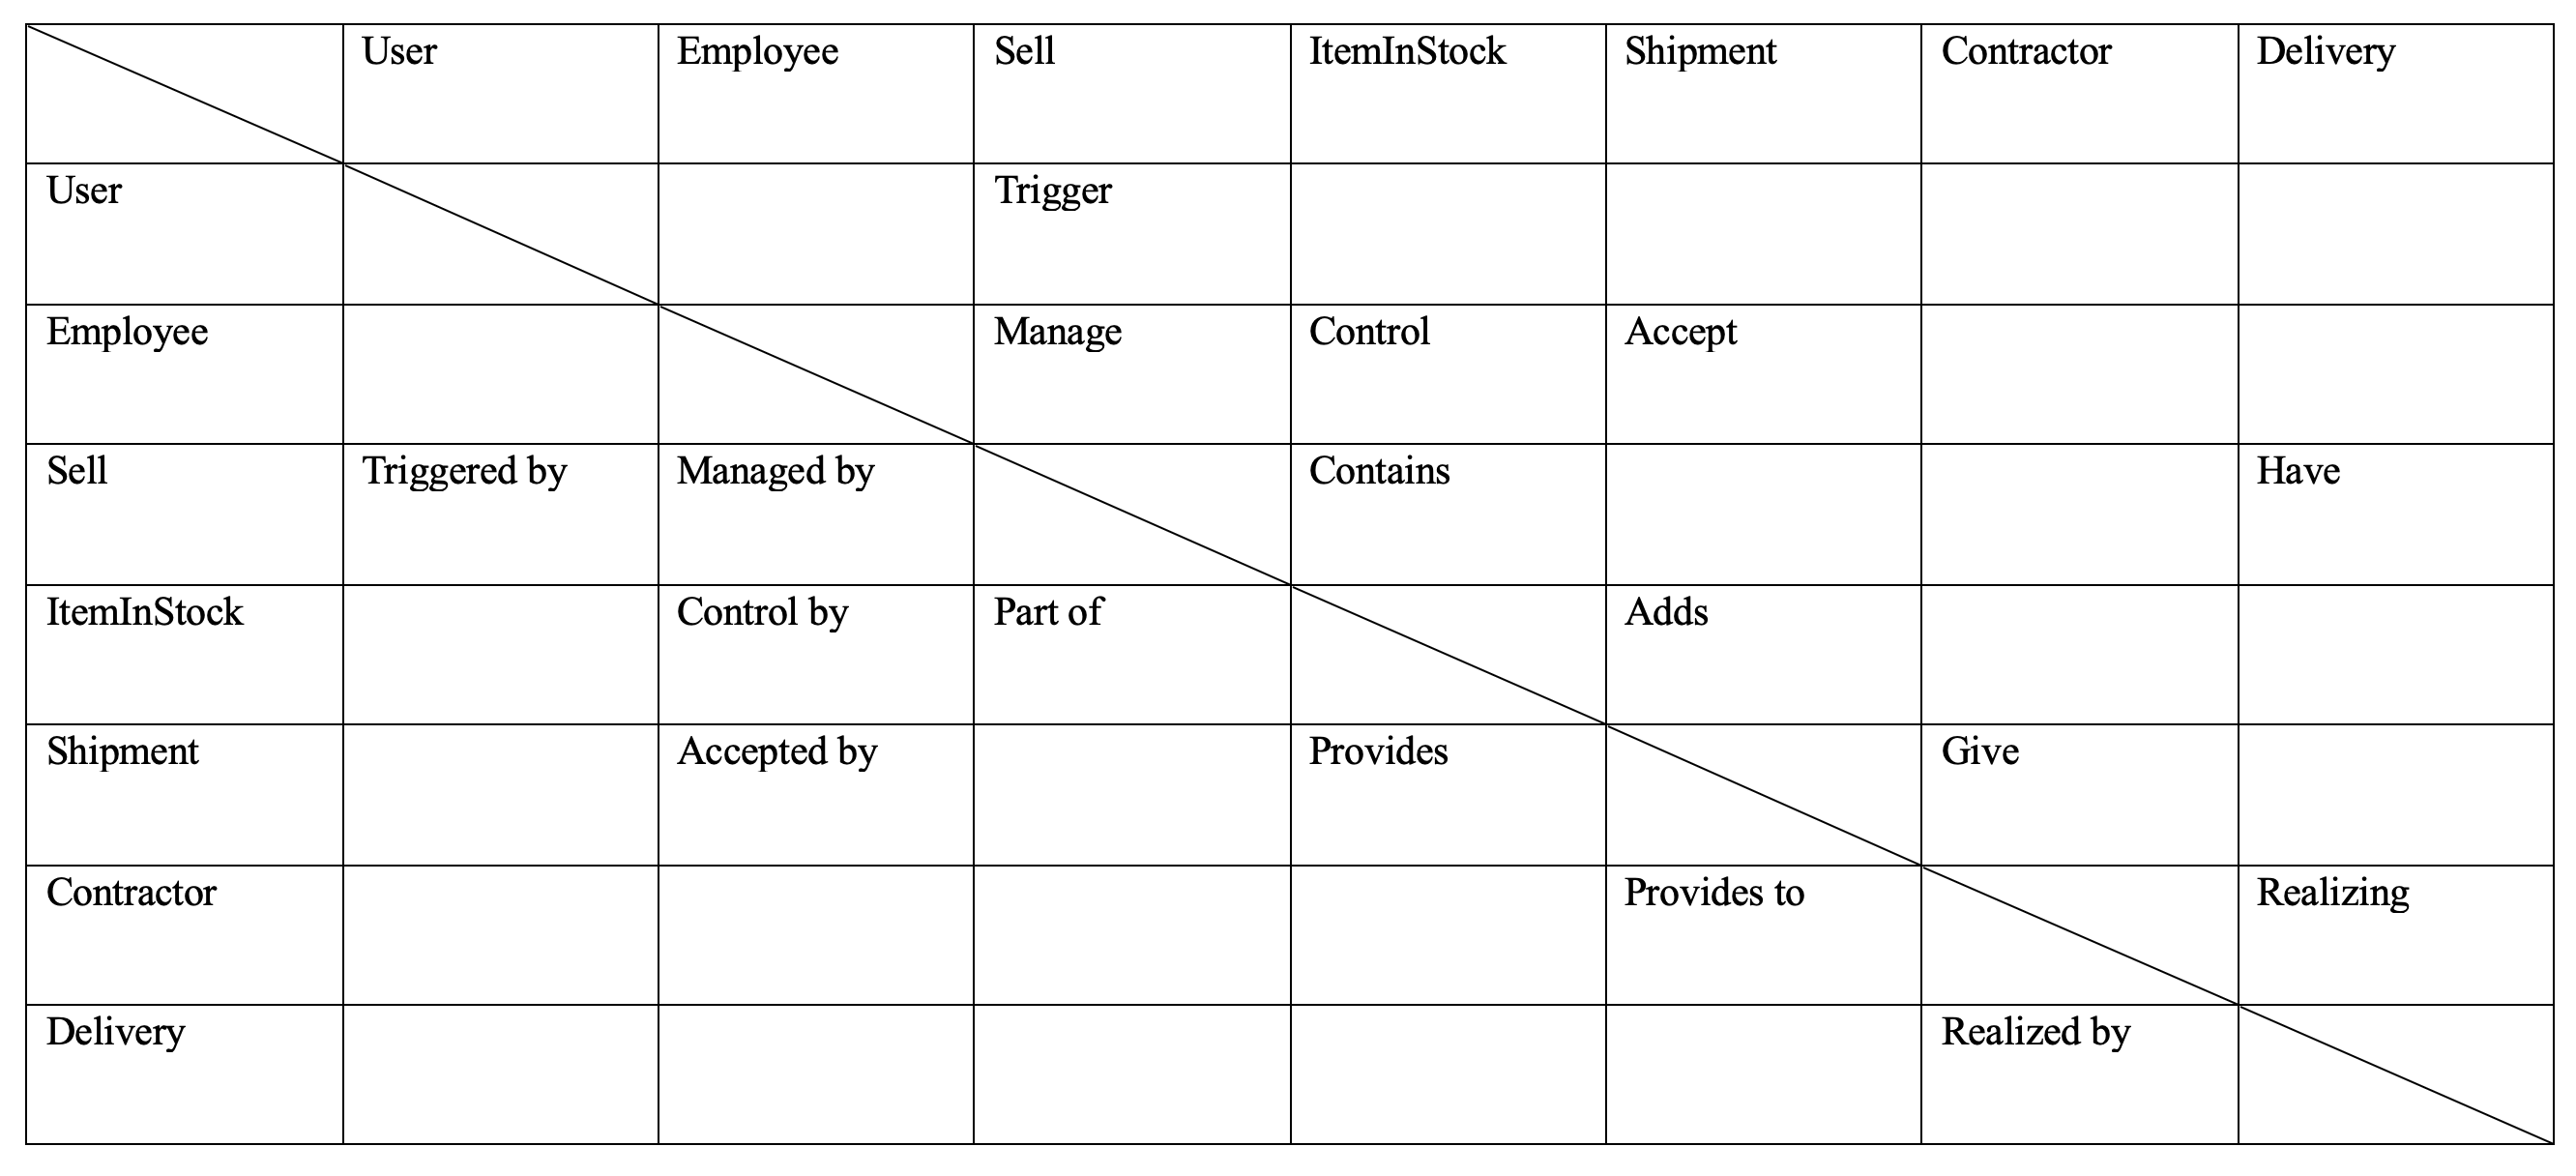
\includegraphics{talbe_of_relations.png}}
        \caption{Таблица связей сущностей.}
        \label{pic1} 
       \end{figure}
    \end{landscape}

\chapter{Логическое проектирование.}
    В процессе выполнения логического проектирования и построения ERD диаграммы были разрешены связи многие-ко-многим при помощи %
    сущностей пересечения. В частности связь многие-ко-многим в отношении Продажи и предметов в магазине. Была проведена нормализация данных, в частности для% 
    таблицы документов, котрые были вынесены в отдельные сущности для ускорения работы базы данных, так как электронные копии документов храняться в <<BLOB>>.

    Для таблиц <<ItmesInShipment>> и <<ItemsInstock>> была произведена восходящая денормалиция с внесением поля <<product\_name>> в таблицу <<ItemsInStock>>.


    
    
    \begin{figure}[H]%current location
        \centering
        \scalebox{0.30}{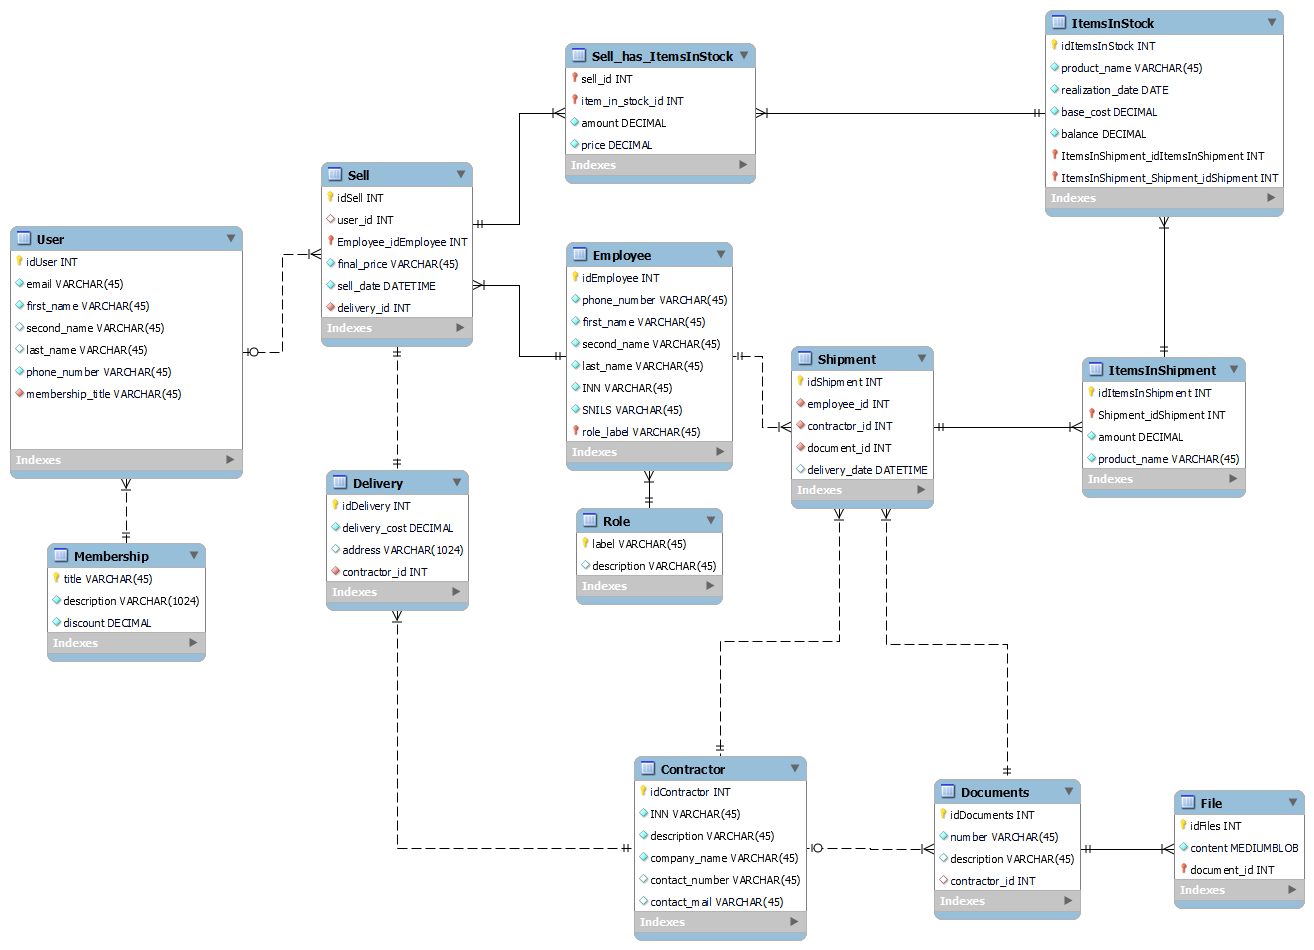
\includegraphics{db_schema.png}}
        \caption{ERR-диаграмма.}
        \label{ERR} 
       \end{figure}


\chapter{Преобразование логической модели в физическую}

\section{Создание физической базы данных}

    Для создания базы данных была применена технология контейнеризации, для запуска базы данных внутри контейнера.%
    Листинг контейнера приведен ниже \ref{docker}.
    
    

    \begin{figure}[H]
        \begin{verbatim}
            version: '3.1'
            services:
            db:
                image: mysql
                restart: always
                ports:
                - "3306:3306"
                environment:
                MYSQL_ROOT_PASSWORD: maindb
                MYSQL_DATABASE: maindb
                MYSQL_USER: maindb
                MYSQL_PASSWORD: maindb
                volumes:
                - ./dbdata:/var/lib/mysq
        \end{verbatim}
        \caption{Листинг YML-файла <<docker-compose.yml>>}
        \label{docker}
    \end{figure}

    После старта рабты контейнера к нему возможно подлючиться средствами <<MySqlWorkbench>> или аналогичным ПО. %
    В нашем случае было принято решение использовать <<Datagrip>>. Процесс создания базы данных изображен на рисунке ниже \ref{create_db}.

    \begin{figure}[H]%current location
        \centering
        \scalebox{0.30}{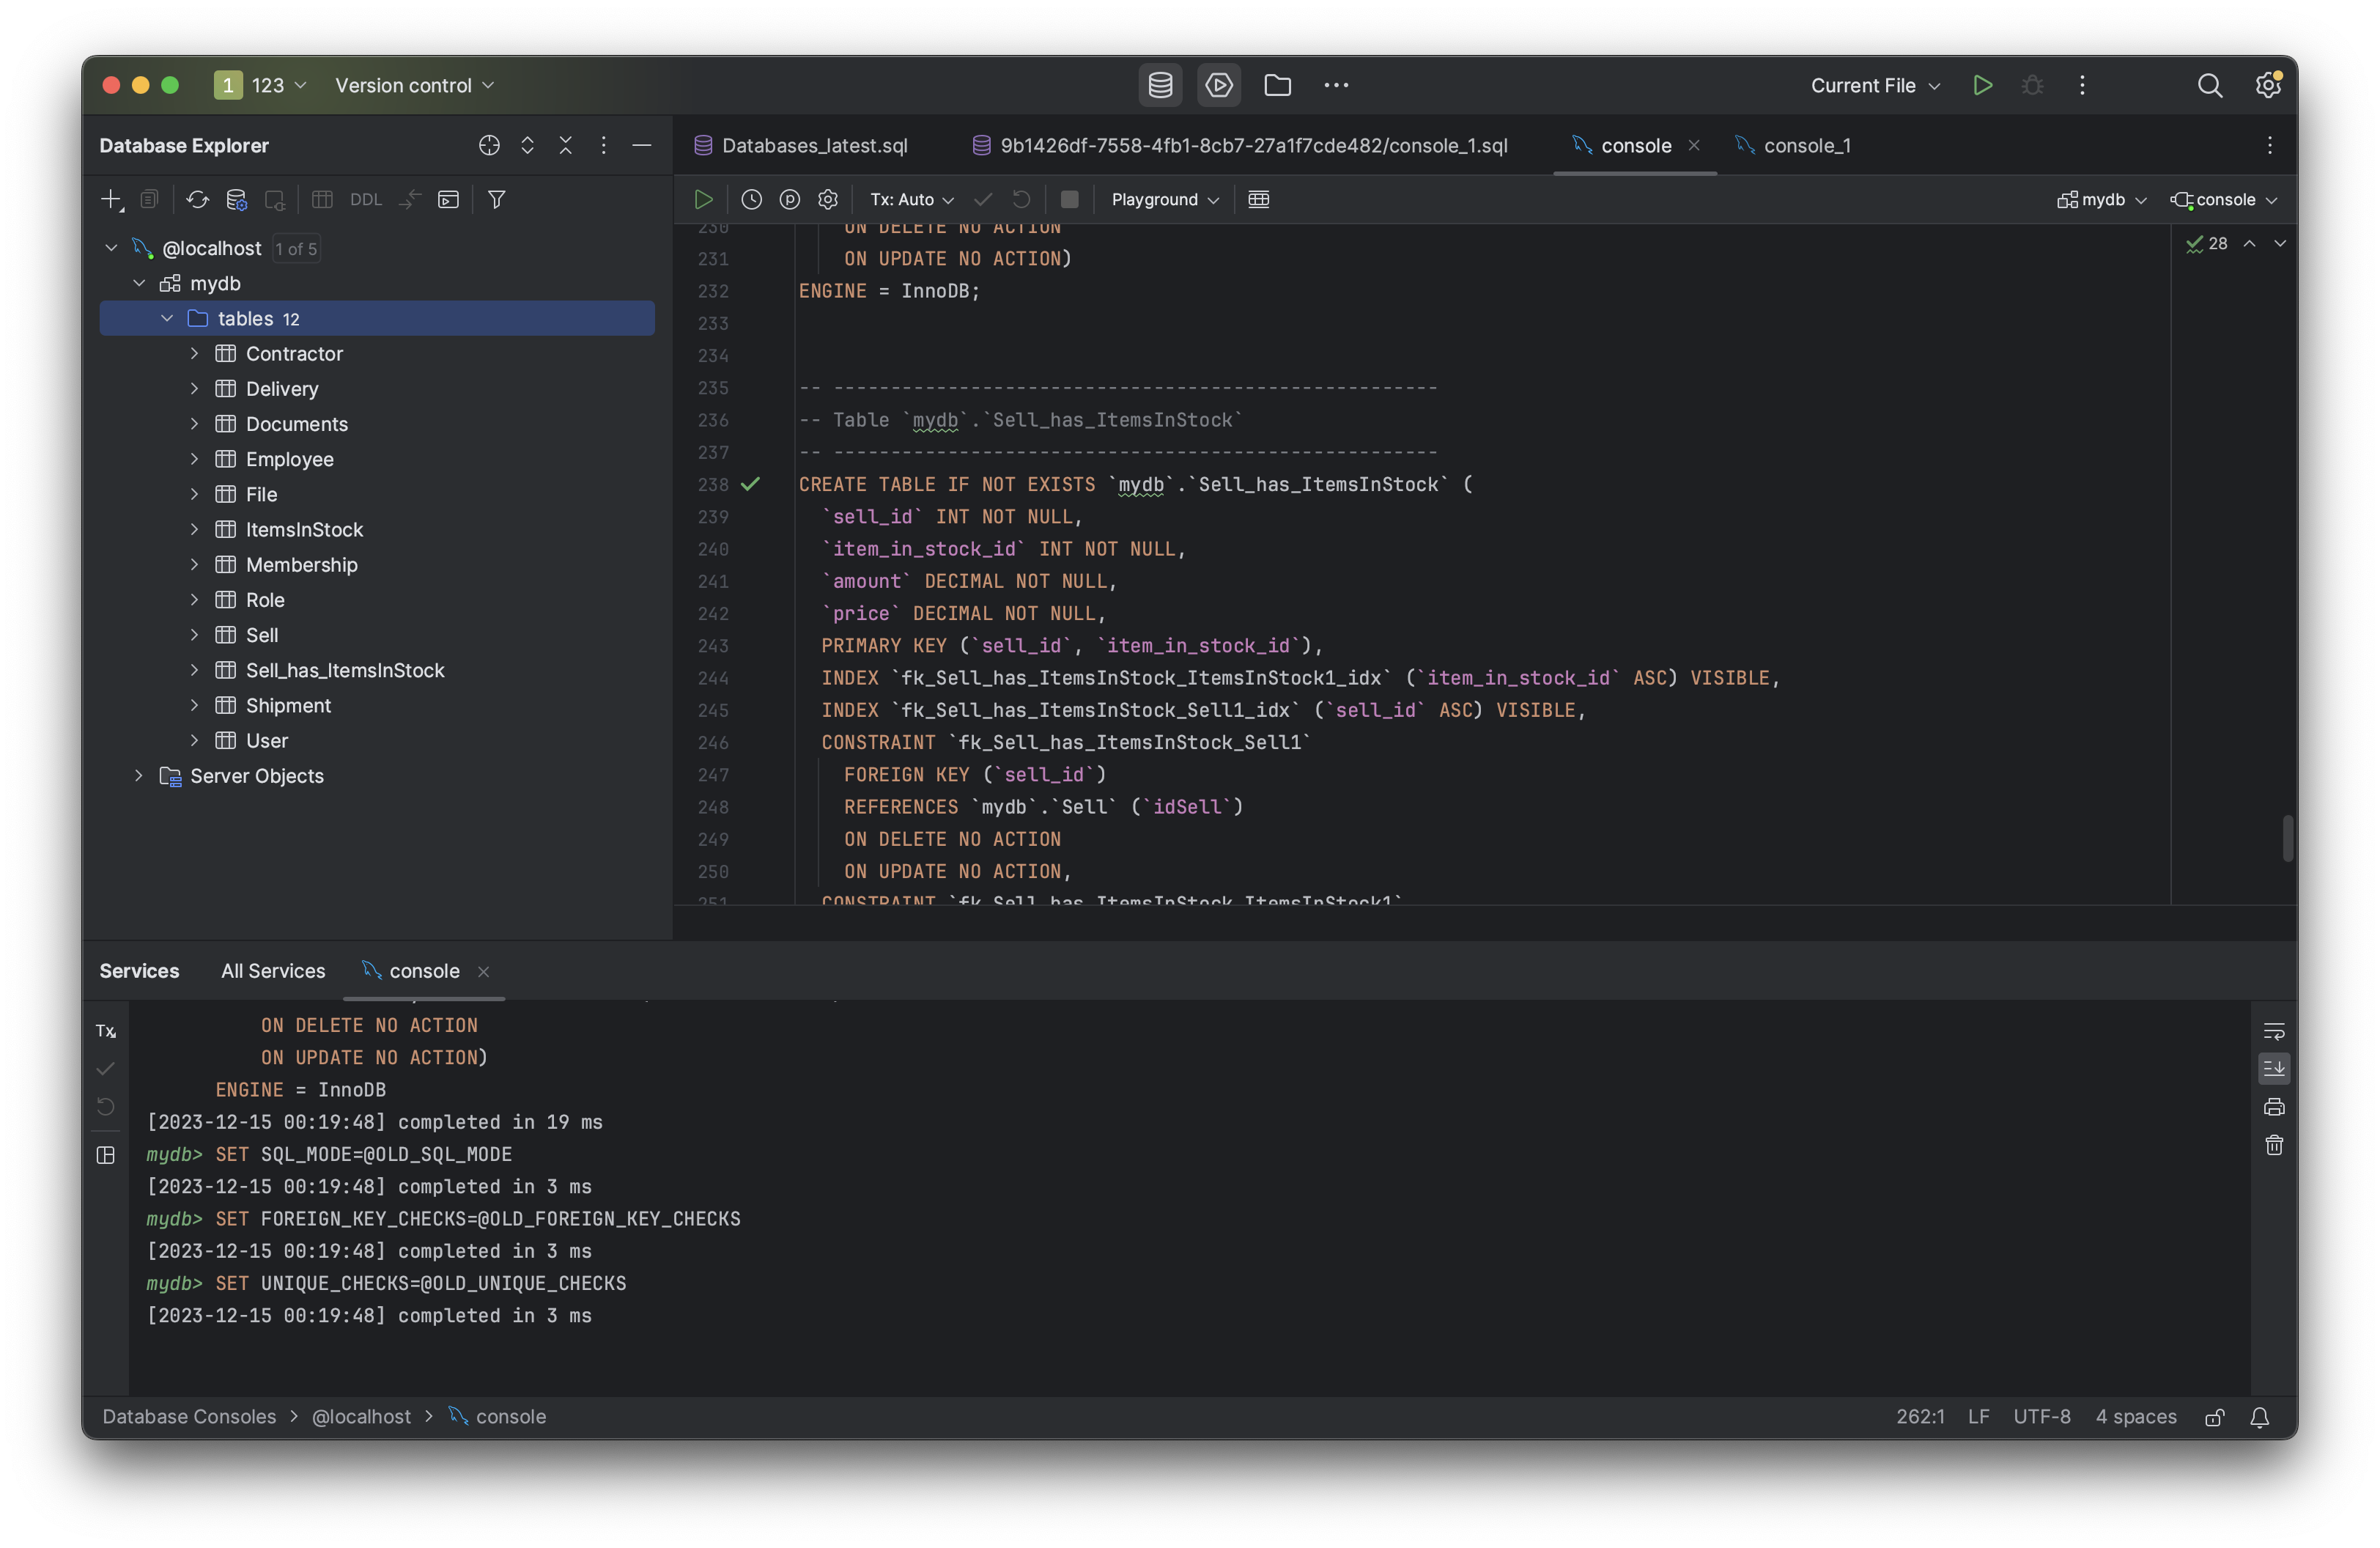
\includegraphics{create_db.png}}
        \caption{ERR-диаграмма.}
        \label{create_db} 
    \end{figure}


    
\section{Создание SQL запросов}
    В данном разделе приведены SQL запросы для получения информации из базы данных

    
        1. Получение всех заказов на доставку, которые были подтверждены определенным сотрудником.
            \begin{center}
                \begin{verbatim}
                SELECT * FROM Delivery
                INNER JOIN Employee
                ON Delivery.employee_id = Employee.idEmployee
                WHERE Employee.first_name = [ИМЯ_СОТРУДНИКА]
                AND
                Employee.last_name = [ФАМИЛИЯ_СОТРУДНИКА];
                \end{verbatim}
            \end{center}
        2. Получение товаров на складе у которых истекла дата реализации.
            \begin{center}
                \begin{verbatim}
                    SELECT * FROM ItemsInStock
                    WHERE realization_date < CURRENT_DATE;

                \end{verbatim}
            \end{center}
        
        3. Получение заявок на доставку которая была принята определенным подрядчиком.
            
                \begin{verbatim}
                    SELECT * FROM Delivery
                    INNER JOIN Contractor
                    ON Delivery.contractor_id=Contractor.idContractor
                    WHERE Contractor.INN = [ИНН_подрядчика];
                \end{verbatim}
            
        
        4. Удаление позиций на складке, чей срок реализации истек.
            \begin{center}
                \begin{verbatim}
                    DELETE FROM ItemsInStock
                    WHERE realization_date < CURRENT_DATE;
                \end{verbatim}
            \end{center}
        
        
        5. Создание заказа с выбранными пользователем позициями.

        \begin{verbatim}

        DECLARE @amount DECIMAL(10, 2) = 0;

        INSERT INTO Sell (final_price) 
        VALUES 
            (@amount);

        SELECT 
            @amount := SUM(price * amount) 
        FROM 
            Sell_has_ItemsInStock 
        WHERE 
            sell_id = [ID_ЗАКАЗА];

        \end{verbatim}


\conclusions{}

В ходе выполнения работ по созданию базы данных для магазина овощей и фруктов были выделены и учтены все бизнес-правила, что позволяет эффективно и качественно управлять данными о выбранных товарами и сложностями их реализации.

Основной упор в проектировании базы данных был сделан на гибкость и возможность изменения условий использования программы лояльности. Была создана структура базы данных, учитывающая все технические и функциональные требования к системе учета лояльности, а также интеграцию с другими компонентами электронного документооборота и отслеживания сроков реализации продукции.

В рамках реализации функционала электронного документооборота была создана форма электронного документа, которая позволяет оперативно и удобно вносить, хранить и обрабатывать данные о реализации продукции. Также было обеспечено автоматическое формирование различных отчетов и документов, что позволяет сократить время на выполнение рутинных операций.

Функционал отслеживания сроков реализации продукции позволяет оперативно контролировать соответствие товаров установленным срокам годности и своевременно принимать решения о дальнейшей судьбе продукта (упаковка в сокращенные сроки реализации или утилизация).

В результате успешной реализации поставленных задач, цель данной работы была достигнута. Все работы были выполнены в полном объеме и с учетом всех требований и пожеланий заказчика. Созданная база данных и функционал программы лояльности позволят эффективно управлять всей цепочкой поставок, реализацией и учетом овощей и фруктов в магазине.

Полученные результаты работы позволят заказчику сократить время и ресурсы, затрачиваемые на ведение учета, отслеживание сроков годности и контроль над реализацией продукции. Кроме того, система электронного документооборота значительно упростит процессы обмена информацией между поставщиками и магазином, а также позволит увеличить прозрачность и надежность этих процессов.

Таким образом, выполнение данной работы было успешным и позволило достичь поставленных целей. Созданная база данных и внедренные функциональные возможности позволят управлять всеми процессами, связанными с овощами и фруктами в магазине, повышая эффективность и надежность бизнес-процессов и упрощая учетную и аналитическую работу.

\newpage

\begin{thebibliography}{10}
    \bibitem{bib1} MySqlWorkbench: официальный сайт. - URL: \url{https://www.mysql.com/products/workbench/} (Дата обращения 15.12.2023)
    \bibitem{bib2} DataGrip: официальный сайт. - URL: \url{https://www.jetbrains.com/ru-ru/datagrip/} (Дата обращения 15.12.2023)
    \bibitem{bib3} Интернет-торговля (рынок России): статья [Электронный ресурс]. – URL: \url{https://www.tadviser.ru/index.php/%D0%A1%D1%82%D0%B0%D1%82%D1%8C%D1%8F:%D0%98%D0%BD%D1%82%D0%B5%D1%80%D0%BD%D0%B5%D1%82-%D1%82%D0%BE%D1%80%D0%B3%D0%BE%D0%B2%D0%BB%D1%8F_%28%D1%80%D1%8B%D0%BD%D0%BE%D0%BA_%D0%A0%D0%BE%D1%81%D1%81%D0%B8%D0%B8%29} (дата обращения 07.11.2023).
    \bibitem{bib4} Приложение к решению Ученого совета Университета ИТМО от «29» ноября 2022 г. № 15 «ТРЕБОВАНИЯ К ВЫПУСКНЫМ КВАЛИФИКАЦИОННЫМ РАБОТАМ». – URL: \url{https://student.itmo.ru/files/1314} (дата обращения 16.03.2023).

\end{thebibliography}

\end{document} 
